%preamble
\documentclass[letterpaper]{article}
\synctex=1
\usepackage{graphicx}
\graphicspath{ {images/} }

\usepackage{lipsum}
\usepackage{float}
% \bibliographystyle{IEEEtran}
% \bibliographystyle{ieeetr}

\usepackage{amssymb}

\usepackage{siunitx}

\usepackage{multirow}
% for merging table cells I think

\usepackage{fancyhdr} %header
\fancyhf{}
\fancyhead[R]{Arun Woosaree XXXXXXX}
\renewcommand\headrulewidth{0pt}
\fancyfoot[C]{\thepage}
\renewcommand\footrulewidth{0pt}
\pagestyle{fancy}

% make subsection use letters
\renewcommand{\thesubsection}{\thesection.\alph{subsection}}


\usepackage{amsthm}
\newtheorem*{clt}{Central Limit Theorem}

%actual document
\begin{document}

% \maketitle %insert titlepage here
\begin{titlepage}
 \begin{center}
  \vspace*{1cm}
  \Huge
  Stat 235
  \vspace{1cm}
  
  Lab 4
  \vspace{1cm}
  
  WOOSAREE, Arun
  \vspace{1cm}
  
  \Huge
  Lab EL12
  \vspace{1cm}
  
  TA: Jessa Marley
  \vspace{1cm}
  
  \today
  \vfill
 \end{center}
\end{titlepage}

\section{}%1

\section{}%2

\subsection{}%2a

\subsection{}%2b

\subsection{}%2c

\section{}%3

\subsection{}%3a

\subsection{}%3b

\section{}%4

\subsection{}%4a

\subsection{}%4b

\subsection{}%4c

\subsection{}%4d

\section{}%5

\subsection{}%5a

% \begin{figure}[H]
%  \centering
%  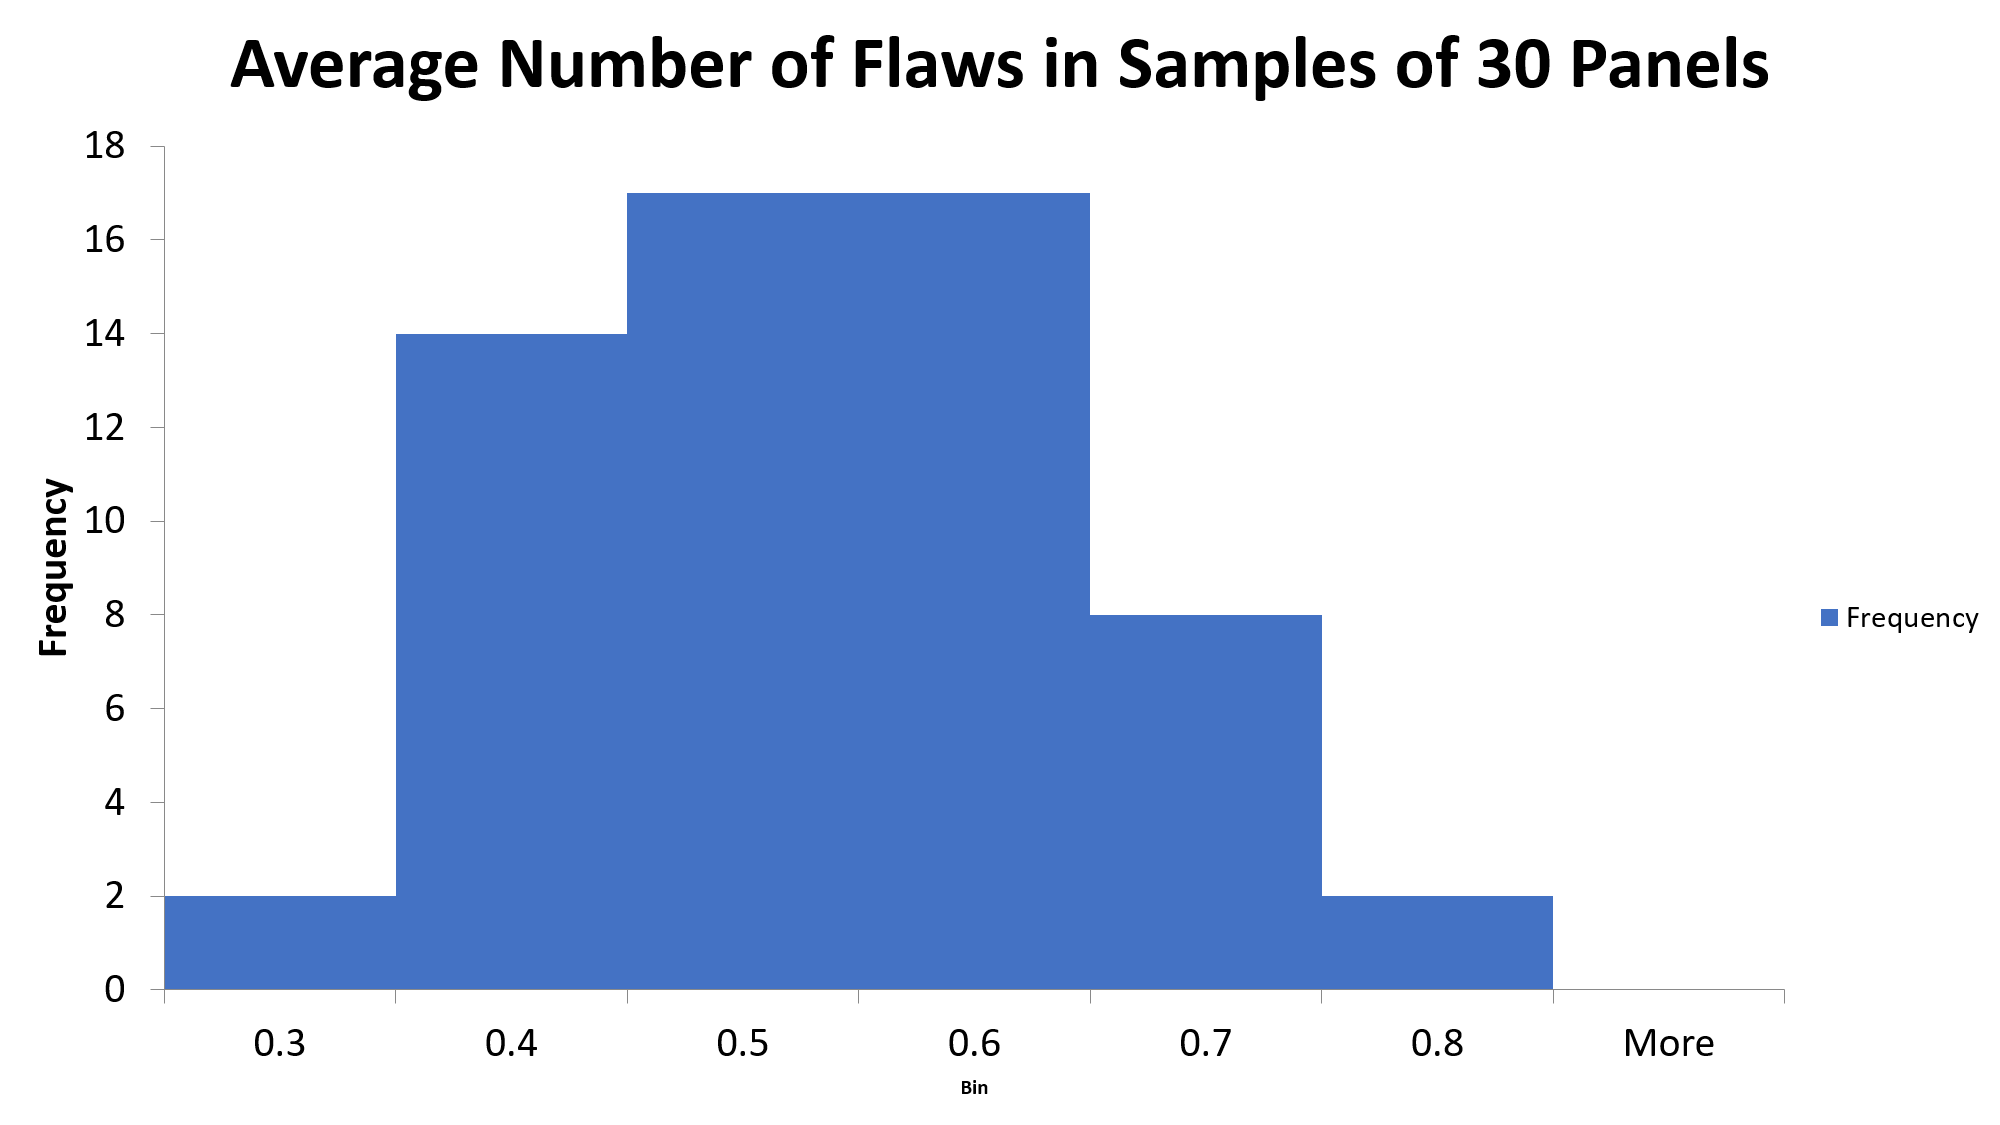
\includegraphics[width=\textwidth]{q5.png}
%  \caption{Average number of flaws in samples of 30 panels from 1800 plastic panels.}
%  \label{5a}
% \end{figure}


\subsection{}%5b


\end{document}
